\section{Motivation} %1.1
The motivation for doing this project contains a vision of restructuring and sustainability of energy in the future.
\subsection{Problems in the Grid}
\subsubsection{Energy Crisis}
The energy crisis is one of the most essential and critical crises in the 21st century. Nowadays, non-renewable resource still consists of a large proportion in the energy system. Non-renewable resource, or finite resource, is depleting. Although we might not meet the complete depletion of non-renewable resources in the future 50 years, based on Hotelling’s "Economics of Exhaustible Resources", David Ricardo proposed that \cite{devarajan1981hotelling} as the historical production stock accumulates, higher grade ores get depleted and the producer resorts to lower grade ores, sustaining greater extraction costs. It means, the extraction costs rise, and the price of the products based on ores rise. Thus, we can assume that the price of most of the non-renewable resources, like oil, coal and gas, rise since these have similar properties with ores. 

\subsubsection{Climate Change}
According to the paper from Nature, \cite{parmesan2003globally} climate change happened in the past 70 years. It has already had effects on the environment around us. Glaciers are shrinking and ices are breaking up earlier on the lakes and rivers. Most climate scientists agree that \cite{epic337530} it is the human expansion that causes the global warming. As we know, carbon dioxide (CO2) is a significant component of the atmosphere. \cite{epic337530} Atmospheric CO2 concentration has been increased by more than a third since the Industrial Revolution began. More importantly, atmospheric carbon dioxide has exceeded the highest level in the past 400,000 years. 

\begin{figure}[t]
\center
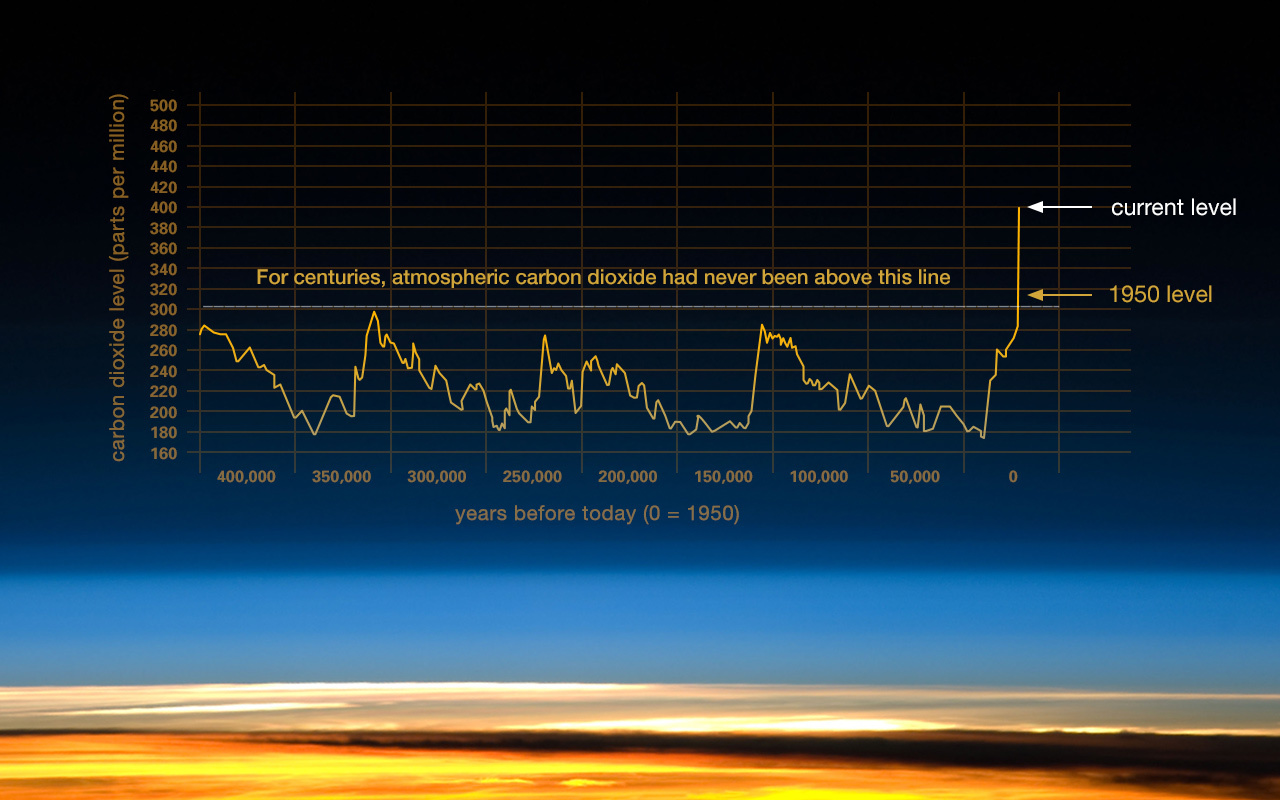
\includegraphics[scale=0.33]{figure/1_1_1_nasa_co2.jpeg}
\longcaption{The evidence that atmospheric CO2 has increased since the Industrial Revolution began}{\label{1_1_1_nasa_co2} The evidence that atmospheric CO2 has increased since the Industrial Revolution began. Image courtesy: https://climate.nasa.gov/evidence}
\end{figure}

\subsubsection{Conflicts and Wars}
An unbalanced energy distribution causes conflicts and wars. The wars, like Gulf War, are more or less derived from energy issues since WW2. 

\subsubsection{Power Interruption}
With the use of unreliable electrical grids, power interruption occurs especially when a natural disaster, such as typhoon, earthquake, and wildfire, happens. Smart grids are more reliable than traditional grids. It’s possible to be build a dynamic technology, like Secondary Frequency Control (SFC), that grid operators need. Self-healing is possible when the storms hit, or physical attack occurs. Therefore, consumers do not encounter power interruptions. 

\subsubsection{Equal Rights to Use Natural Power}
Everyone should have his/her right to use natural resources equally. However, in most countries, the fact is that a few large companies dominate public funds and gradually form a monopoly market. Entrepreneurs use their centralised power to restrict consumers’ right to disagree. 

Technologies should begin with the customers. It is connected with intelligent devices that always communicate with each other. The system creates and stores energy throughout the day and any extra energy flows back onto the grid to power neighbours and businesses. Those smart energy buildings will then power the entire communities. It’s fairly distributed, clean, and more cost-effective. 

\subsubsection{New Issues from Clean Energy}
Using clean energy from renewable resource could be one of the ways to solve the problems above! In fact, recently, California Assembly passed a bill requiring 100 percent of the state’s electricity to come from carbon-free sources by the end of 2045. In China and Germany, renewables are outgrowing their grids. The public is accepting the idea of using electric cars instead of fuel cars. 

However, these renewable energy sources which interfaced with national or state power systems has introduced new issues on stability, resilience, and reliability. Thus, power networks are under modification.\\

For countries like Switzerland, where 62\% of electricity comes from renewable sources, it’s another situation. Although it’s really friendly to the environment, energy instability has also increased. Sun doesn’t always shine, wind doesn’t always blow, and water doesn’t always flow. 

\subsection{Solution: Secondary Frequency Control}
As these highly variable sources come to represent a growing portion of the grid, it becomes more and more important to develop an accurate and validated model to represent these units in the computational tools used to analyse the ancillary services of smart grids.\\

Smart grid powers the modern city, and Secondary Frequency Control is one of the most important parts in smart grids to ensure the energy security in electricity systems and to allow the increasing renewable energy penetration. Secondary Frequency Control ensures the frequency of the electricity network is always restored to its nominal value when disturbances occur in the system. The frequency is one of the key “health” indicators of smart grids. Actively monitoring and controlling can ensure system security. This is done by remotely controlling the power output of generating units (both conventional and renewables) through a communication network. 